\documentclass[presentation]{beamer}

\usepackage{tikz}
\usetikzlibrary{positioning,calc}
\usetikzlibrary{shapes.geometric}
\usetikzlibrary{backgrounds}% only to show the bounding box
\usetikzlibrary{shapes,arrows}
\usepackage{pgfplots}
\usepackage{pgfplotstable}
\usetikzlibrary{pgfplots.groupplots}
\pgfplotsset{compat=1.12}
\usepackage{appendixnumberbeamer}
\usepackage{amsmath}
\date{27th March 2017}
\usetheme{ometropolis}

\metroset{progressbar=frametitle}

\pgfplotscreateplotcyclelist{decent cycle}{%
  {blue, mark=*, mark options={fill=blue},
    mark size=2pt},
  {cyan, mark=square*, mark options={fill=cyan},
    mark size=2pt},
  {magenta, mark=triangle*, mark options={fill=magenta},
    mark size=3pt},
  {blue, mark=*, mark options={fill=blue},
    mark size=2pt},
  {cyan, mark=square*, mark options={fill=cyan},
    mark size=2pt},
  {magenta, mark=triangle*, mark options={fill=magenta},
    mark size=3pt},
}

\pgfplotsset{
  decent/.style={
    cycle list name=decent cycle,
  }
}
\renewcommand{\vec}[1]{\ensuremath{\boldsymbol{#1}}}
\newcommand{\ddt}[1]{\frac{\partial #1}{\partial t}}
\newcommand{\zhat}{\hat{\vec{z}}}
\newcommand{\W}{\ensuremath{\mathbb{W}}}

\DeclareMathOperator{\grad}{grad}
\let\div\relax
\DeclareMathOperator{\div}{div}
\DeclareMathOperator{\curl}{curl}
\newcommand{\vsubset}[1]{\rotatebox[origin=c]{90}{\ensuremath{\subset}}}
\newcommand{\inner}[2]{\ensuremath{\langle #1, #2 \rangle}}
\author{Lawrence Mitchell\inst{1}}
\institute{
\inst{1}Departments of Computing and Mathematics, Imperial College
London
}

\graphicspath{{./\jobname.figures/}}

\newcommand{\arxivlink}[2]{%
  \href{http://www.arxiv.org/abs/#1}%
  {{\small\texttt{arXiv:\,#1\,[#2]}}}%
}
\newcommand{\doilink}[1]{%
  \href{http://dx.doi.org/#1}%
  {{\small\texttt{doi:\,#1}{}}}%
}
\usepackage[url=false,
            doi=true,
            isbn=false,
            style=authoryear,
            firstinits=true,
            uniquename=init,
            backend=biber]{biblatex}

\setbeamertemplate{bibliography item}{}
\renewcommand{\bibfont}{\footnotesize}
\addbibresource{references.bib}

\setlength{\bibitemsep}{1ex}

\renewbibmacro{in:}{}
\DeclareFieldFormat[article]{volume}{\textbf{#1}}
\DeclareFieldFormat{doi}{%
  doi\addcolon%
  {\scriptsize\ifhyperref{\href{http://dx.doi.org/#1}{\nolinkurl{#1}}}
    {\nolinkurl{#1}}}}
\AtEveryBibitem{%
\clearfield{pages}%
\clearfield{issue}%
\clearfield{number}%
}

\usepackage{minted}
\usepackage{cancel}
\title{From here to there}
\subtitle{challenges for \cancel{peta} exa-scale transient simulation}

\begin{document}

\maketitle

\begin{frame}
  \frametitle{What we all would like for exascale}
  \begin{center}
    \Large High frequency, single-core CPUs
  \end{center}
\end{frame}

\begin{frame}
  \frametitle{What we have to work with}
  \begin{tabular}{lccccc}
    Chip & Cores & TF/s & GB/s & F/B & Power \\
    \hline
    NVidia P100 & 56 (3584) & 5.3 & 730 & 7.2 & 250 (21 GF/W) \\
    Xeon Phi 7290F & 72 & 3.5 & 450 & 7.8 & 260 (13 GF/W) \\
    Broadwell & 22 & 0.78 & 150 & 5.2 & 140 (5.6 GF/W)
  \end{tabular}

  \begin{block}{Exascale}
    Easy, just multiply by $10^6$.
    \begin{itemize}
    \item<1-> 190K NVidia P100s, 1e9-way concurrency, 50MW
    \item<1-> 290K Intel Phis, 1e8-way concurrency, 75MW
    \item<1-> 1.3M Intel Broadwells, 3e7-way concurrency, 180MW
    \item<2-> 1 Boeing 747, 140MW
    \item<3-> 1 Sizewell B, 1200MW
    \end{itemize}
  \end{block}
  % NVIDIA P100 (Pascal) 56 SMTs 5.3TF/s 732GB/s (16GB) 7.2F/B 250W 21F/W

  % Intel Xeon Phi 7290F 72 cores 3.5TF/s ~450GB/s (16GB) 7.8F/B 260W 13F/W

  % Intel Broadwell E5-2699v4 22 cores 0.78TF/s 150GB/s (<1.5TB) 5.2F/B
  % 140W 5.6F/W
\end{frame}
\begin{frame}
  \frametitle{How do you achieve these numbers?}

  \begin{onlyenv}<1>
    \begin{center}
      \Large
      Run LINPACK
  \end{center}
  \end{onlyenv}

  \begin{onlyenv}<2>
    \begin{itemize}
    \item Do many calculations on data when you fetch it (flops are free)
    \item Do the same calculation on adjacent data items (vectorise)
    \item Avoid communicating (hah!)
    \end{itemize}
  \end{onlyenv}
\end{frame}

\begin{frame}
  \frametitle{How do I know what is good?}

  \begin{block}{Build a model \parencite{Fischer:2015}}
    Problem size $N$, processes $P$.
    \begin{equation*}
      T(N, P) = \max{(T_a(N, P), T_c(N, P))} + c
    \end{equation*}
    \begin{itemize}
    \item $T_a(N, P) = T_a(N, 1)/P$ parallelizable work
    \item $T_c$ communication
    \item $c$ non-parallelizable
    \end{itemize}
  \end{block}
  \begin{center}
    \begin{columns}
      \begin{column}{0.4\textwidth}
        \begin{block}{Strong scaling}
          Fix $N$, increase $P$.
        \end{block}
      \end{column}
      \begin{column}{0.4\textwidth}
        \begin{block}{Weak scaling}
          Fix $N/P$, increase $P$.
        \end{block}
      \end{column}
    \end{columns}
  \end{center}
\end{frame}
\begin{frame}
  \frametitle{Strong scaling}
  This is the important one, since larger transient simulations need
  more timesteps.  To maintain time to solution, must decrease $N/P$
  with increasing $N$.

  \begin{block}{Some costs do not go to zero}
    \begin{itemize}
    \item $\lim_{P\rightarrow \infty} T_a(N, P) = 0$.
    \item $\lim_{P\rightarrow\infty} T_c(N, P) \ne 0$.
    \item Ignore $c$ (reasonable for CPU).
    \item Economics: stop increasing $P$ once $T_a < T_c$ (less than
      50\% efficiency).
    \end{itemize}
  \end{block}
\end{frame}

\begin{frame}
  \frametitle{Simple models}
  \begin{block}{Computation}
    Achieved flop rate for ``atomic'' unit of computation.
    $t_a$ (s/F).  Measure using $P=1$, $N\rightarrow\infty$.
  \end{block}
  \begin{block}{Communication}
    Time (s) to send $m$ doubles
    \begin{equation*}
      t_c(m) = \alpha^* + \beta^* m
    \end{equation*}
    non-dimensionalise, provides comparable machine parameters
    $\alpha = \alpha^*/t_a$ (F), $\beta = \beta^*/t_a$ (F/B).
  \end{block}
\end{frame}

\begin{frame}
  \frametitle{Measure on your machine}
  \begin{columns}
    \begin{column}{0.5\textwidth}
      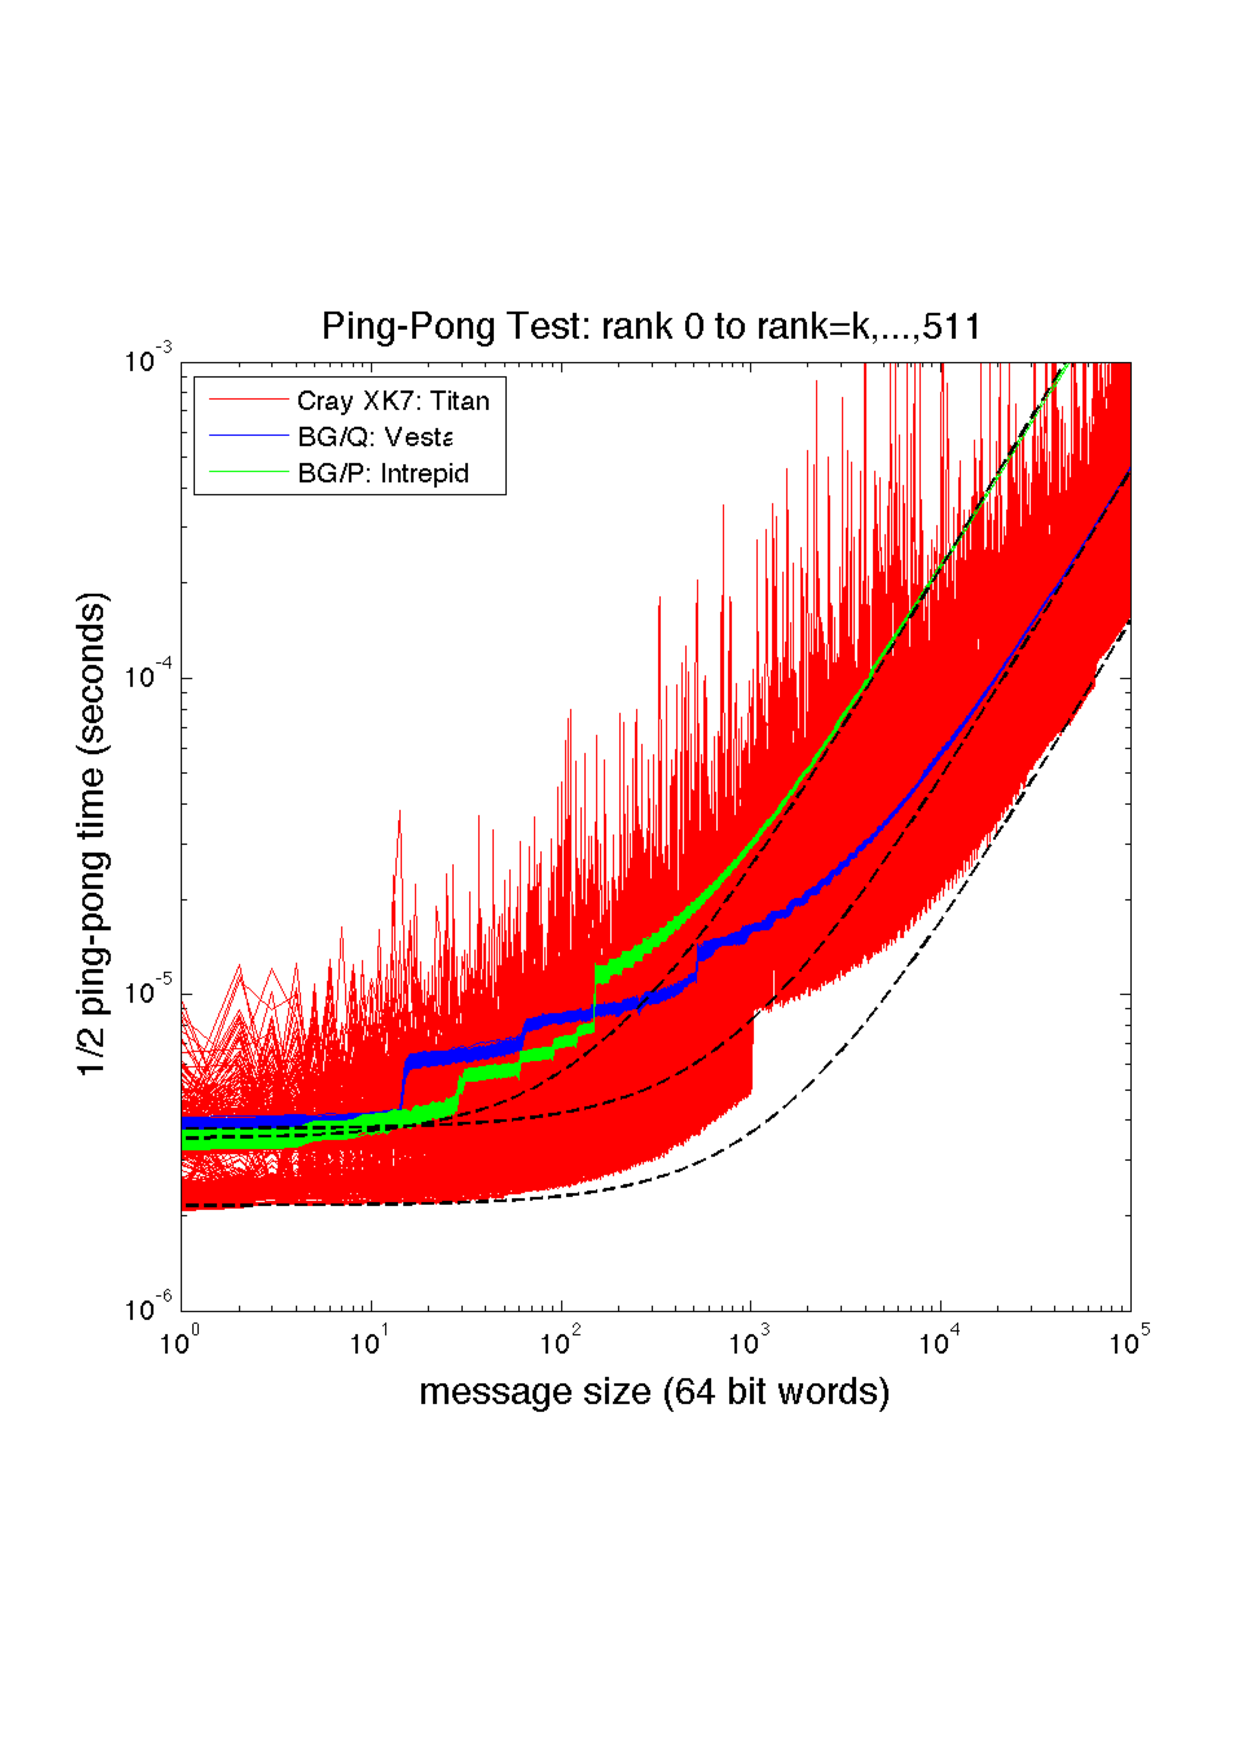
\includegraphics[width=\columnwidth]{ping-pong}
    \end{column}
    \begin{column}{0.5\textwidth}
      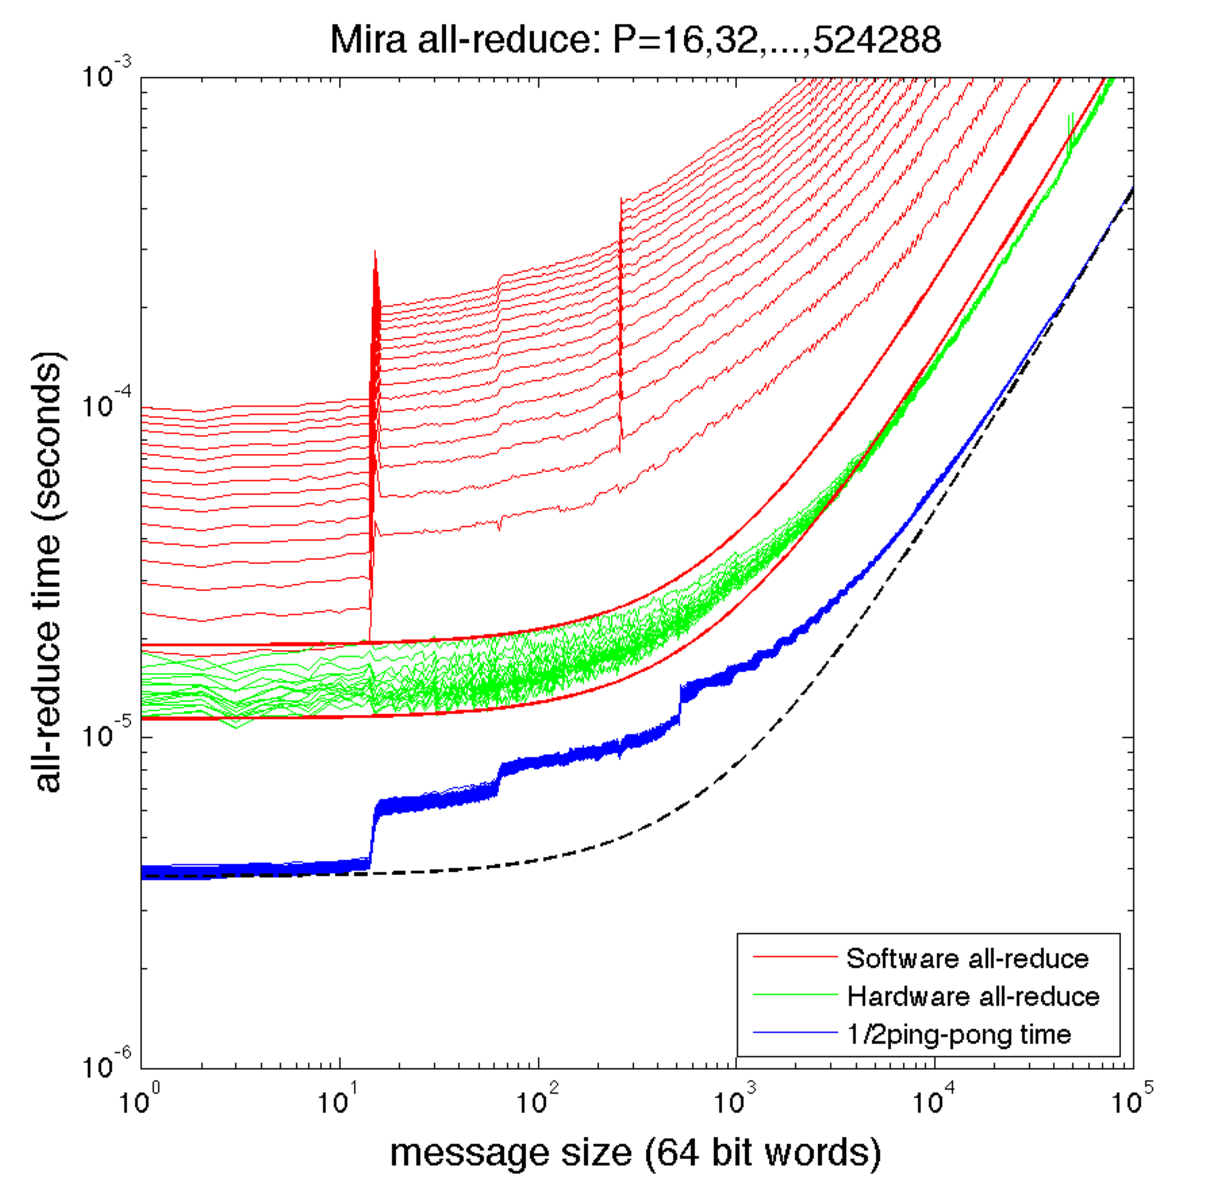
\includegraphics[width=\columnwidth]{allreduce}
    \end{column}
  \end{columns}
\end{frame}

\begin{frame}
  \frametitle{Back to models}

  \begin{block}{Jacobi iteration}
    7-point stencil.

    \begin{itemize}
    \item computation: $T_a = 14 (N/P) t_a$
    \item communication: exchange 6 faces $6 (N/P)^{2/3}$ values.
      $T_c = 6(\alpha + \beta (N/P)^{2/3})t_a$.
    \end{itemize}
    No $P$ dependence (perfectly scalable).

    Measure $\alpha$, $\beta$.  Set $T_a = T_c$, solve for $N/P$.

    e.g. BG/Q $\alpha = 3750$, $\beta = 2.86$

    $N/P \sim 1700$.

    If $\beta = 0$ (infinite bandwidth), $N/P \sim 1600$.
  \end{block}
\end{frame}
\begin{frame}
  \frametitle{Jacobi no good for global solve}
  \begin{block}{Conjugate gradients}
    \begin{itemize}
    \item computation: $T_a/t_a = 27 (N/P)$.
    \item communication: $T_c/t_a = 6(\alpha + \beta(N/P)^{2/3}) +
      2\cdot 2\alpha\log_2 P$.
    \end{itemize}

    $\log P$ factor (not perfectly scalable).

    Set $P=10^6$ gives $N/P \sim 12000$.

    $P=10^9$ gives $N/P \sim 17000$.

    But, remember the BG/Q picture: $2 \alpha \log_2 P \rightarrow 4
    \alpha$.

    $N/P \sim 2100$, even better with a single reduction ($N/P \sim 1500$).
  \end{block}
\end{frame}
\begin{frame}
  \frametitle{How about multigrid?}
  \begin{block}{Multigrid (geometric)}
    \begin{itemize}
    \item computation: $T_a/t_a = 50 (N/P)$.
    \item communication: $T_c / t_a = 8 \alpha \log_2(N/P) + 30
      \beta(N/P)^{2/3} + 4\cdot 2 \alpha \log_2 P$.
    \end{itemize}
    Again, $\log P$ factor prevents perfect scalability.

    $P=10^6$ gives $N/P \sim 21000$.

    $P = 10^9$ gives $N/P \sim 27000$.

    What if the (generalised) tree reduction is constant cost?
    $2\alpha \log_2 P \rightarrow 4 \alpha$.

    $N/P \sim 10000$
  \end{block}
\end{frame}

\begin{frame}
  \frametitle{Latency is all that matters!}

  Things to note

  If $\alpha$ decreases, can strong scale much better

  In strong scaled limit, don't really care about $\beta$ (since data
  moved is small).

  If you can strong scale into cache, everything looks much better
  (bandwidth is higher).  But this is bad for GPUs (need lots of work
  to hide latency).

  If cores get relatively faster, $\alpha, \beta$ increase (can't
  strong scale as well).

  Ask your vendor to spend power on interconnect, not flops?

  Questions for climate?  Columnwise decomposition important for
  numerics.  Does it get in the way of strong scaling? 
  
  Problems:
  - decomposition doesn't provide minimal surface area.
  - Unit of decomposition is 1 column.  C-grid staggering gives ~800
  velocity + pressure dofs.  Adding in additional variables, probably
  more work than strong scaling limit.

  - Suggests distributed memory on socket + shared memory parallel in
  a socket (to scale a bit further: ``message latency'' much reduced).
\end{frame}

\begin{frame}
  \frametitle{Addressing latency}
  What to do?

  Communicate less

  Communicate less frequently
\end{frame}
\appendix
\begin{frame}[t,allowframebreaks]
  \frametitle{References}
  
  \printbibliography[heading=none]
\end{frame}
\end{document}
